% \afterpage{
% \clearpage
% \thispagestyle{empty}
\captionsetup[subfigure]{position=above,labelformat=empty}
% \subfiguretopcaptrue
\begin{figure}[htbp]
    % \centering
% \captionsetup[subfigure]{position=top}        
    % \addtolength{\abovecaptionskip}{20pt}
    \addtolength{\belowcaptionskip}{20pt}
    
\begin{subfigure}{.5\textwidth}
\caption{Scenario a)}
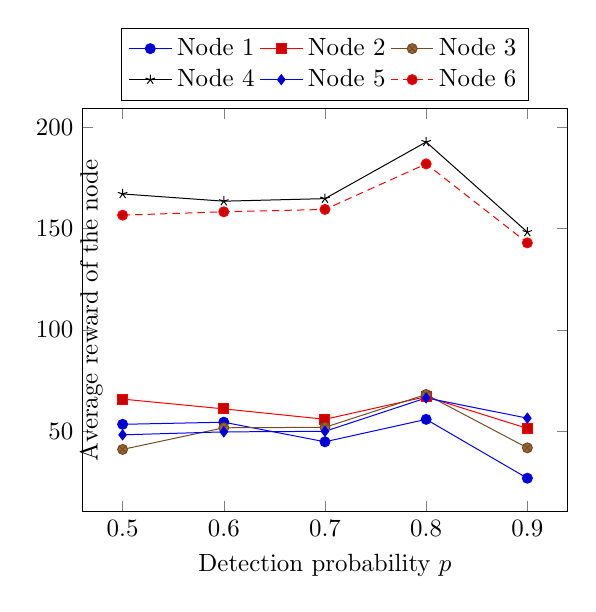
\begin{tikzpicture}[scale=0.9]
\begin{axis}[
  xlabel={Detection probability $p$},
  ylabel={Average reward of the node },
  y label style={at={(0.06,0.5)}},
  xtick={0.5,0.6,0.7,0.8,0.9,1.0},
  legend style={at={(0.5,1.2)},cells={align=right}, anchor=north,legend columns=3},
  grid style=dashed,
]

\addplot+[]
    coordinates {
(0.5,53.3115955435)(0.6,54.3545841648)(0.7,44.6785742262)(0.8,55.7545888625)(0.9,26.6726622755)
};

\addplot+[]
    coordinates {
(0.5,65.7687020142)(0.6,60.9406466924)(0.7,55.8056247195)(0.8,66.9612779492)(0.9,51.2874064555)
};

\addplot+[]
    coordinates {
(0.5,40.908080525)(0.6,51.5966479036)(0.7,51.8294937238)(0.8,68.0588803377)(0.9,41.6899098384)
};

\addplot+[]
    coordinates {
(0.5,167.1425811)(0.6,163.56587834)(0.7,164.826844567)(0.8,192.814744826)(0.9,148.302330965)
};

\addplot+[]
    coordinates {
(0.5,48.1098633801)(0.6,49.569538244)(0.7,49.8423884228)(0.8,66.3485362884)(0.9,56.3535029043)
};

\addplot+[]
    coordinates {
(0.5,156.653749239)(0.6,158.321084535)(0.7,159.485991256)(0.8,181.985919611)(0.9,142.979383044)
};

\legend{Node 1, Node 2, Node 3, Node 4, Node 5, Node 6}
\end{axis}
\end{tikzpicture}
% \label{fig:nodeimp_single}
\end{subfigure}
% \hspace*{\fill}
\begin{subfigure}{.5\textwidth}
\caption{Scenario b)}
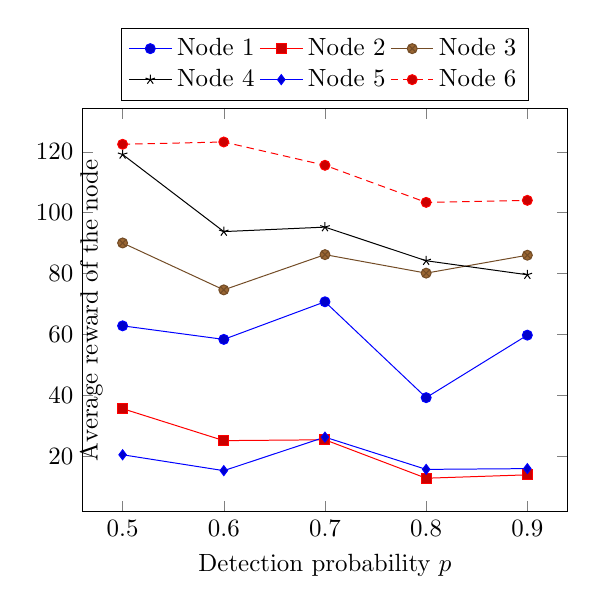
\begin{tikzpicture}[scale=0.9]
\begin{axis}[
  xlabel={Detection probability $p$},
  ylabel={Average reward of the node },
  y label style={at={(0.06,0.5)}},
  xtick={0.5,0.6,0.7,0.8,0.9,1.0},
  legend style={at={(0.5,1.2)},cells={align=right}, anchor=north,legend columns=3},
  grid style=dashed,
]

\addplot+[]
    coordinates {
(0.5,62.8521432343)(0.6,58.3969143024)(0.7,70.7528787794)(0.8,39.262008432)(0.9,59.7930672705)
};

\addplot+[]
    coordinates {
(0.5,35.6477622245)(0.6,25.1466084924)(0.7,25.4245369898)(0.8,12.7966666667)(0.9,13.9088095238)
};

\addplot+[]
    coordinates {
(0.5,90.0722009288)(0.6,74.6625998331)(0.7,86.2388746563)(0.8,80.1605264877)(0.9,86.0444903266)
};

\addplot+[]
    coordinates {
(0.5,119.130037557)(0.6,93.8066520365)(0.7,95.2732464682)(0.8,84.2315618108)(0.9,79.6278821173)
};

\addplot+[]
    coordinates {
(0.5,20.5031617844)(0.6,15.2818516008)(0.7,26.2961789474)(0.8,15.7022412698)(0.9,15.9502350792)
};

\addplot+[]
    coordinates {
(0.5,122.48657341)(0.6,123.23710488)(0.7,115.578393437)(0.8,103.398742076)(0.9,104.070036133)
};

\legend{Node 1, Node 2, Node 3, Node 4, Node 5, Node 6}
\end{axis}
\end{tikzpicture}
% \label{fig:nodeimp_topo1_multiple}
\end{subfigure}
\begin{subfigure}{.5\textwidth}
\caption{Scenario c)}
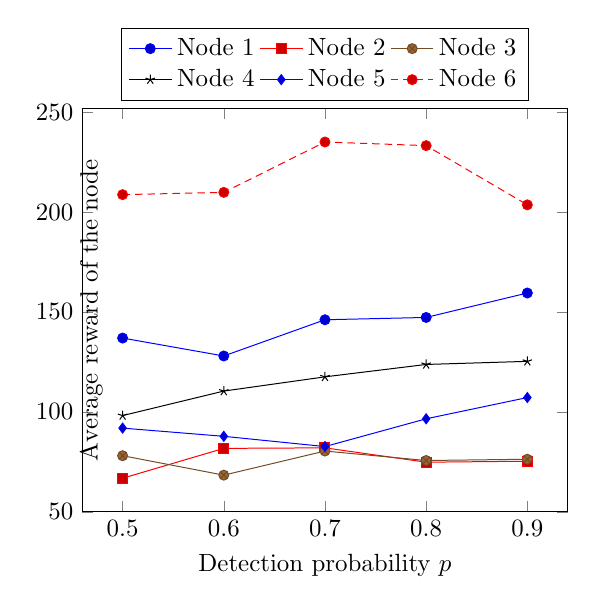
\begin{tikzpicture}[scale=0.9]
\begin{axis}[
  xlabel={Detection probability $p$},
  ylabel={Average reward of the node },
  y label style={at={(0.06,0.5)}},
  xtick={0.5,0.6,0.7,0.8,0.9,1.0},
  legend style={at={(0.5,1.2)},cells={align=right}, anchor=north,legend columns=3},
  grid style=dashed,
]

\addplot+[]
    coordinates {
(0.5,136.927310407)(0.6,127.960388869)(0.7,146.086472254)(0.8,147.235410707)(0.9,159.469537067)
};

\addplot+[]
    coordinates {
(0.5,66.7988560021)(0.6,81.7311837411)(0.7,82.0017291916)(0.8,74.8192160051)(0.9,75.3089759032)
};

\addplot+[]
    coordinates {
(0.5,78.0634438963)(0.6,68.3402801041)(0.7,80.4009699099)(0.8,75.6559526089)(0.9,76.2953944418)
};

\addplot+[]
    coordinates {
(0.5,98.1369317879)(0.6,110.402016785)(0.7,117.520015671)(0.8,123.721254753)(0.9,125.271778646)
};

\addplot+[]
    coordinates {
(0.5,91.8750388819)(0.6,87.764930694)(0.7,82.6400238592)(0.8,96.5305636149)(0.9,107.164379512)
};

\addplot+[]
    coordinates {
(0.5,208.678957661)(0.6,209.815036383)(0.7,235.024736742)(0.8,233.211114765)(0.9,203.573491786)
};

\legend{Node 1, Node 2, Node 3, Node 4, Node 5, Node 6}
\end{axis}
\end{tikzpicture}
\label{fig:nodeimp_topofullmesh_single}
\end{subfigure}
\begin{subfigure}{.5\textwidth}
\caption{Scenario d)}
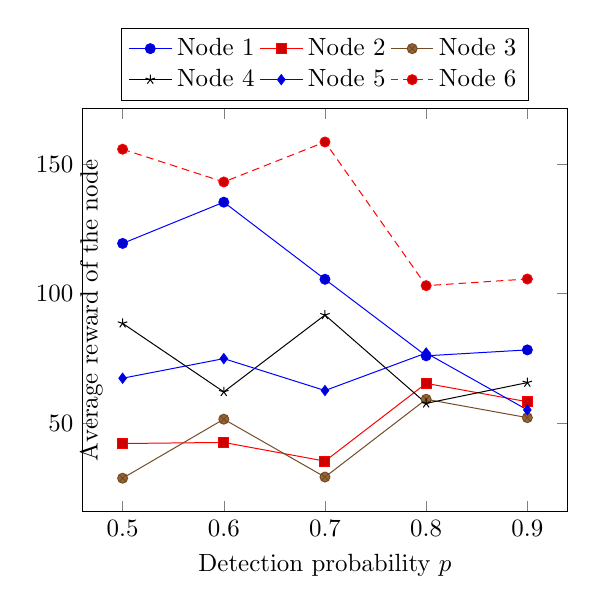
\begin{tikzpicture}[scale=0.9]
\begin{axis}[
  xlabel={Detection probability $p$},
  ylabel={Average reward of the node },
  y label style={at={(0.06,0.5)}},
  xtick={0.5,0.6,0.7,0.8,0.9,1.0},
  legend style={at={(0.5,1.2)},cells={align=right}, anchor=north,legend columns=3},
  grid style=dashed,
]
\addplot+[]
    coordinates {
(0.5,119.371712601)(0.6,135.286667912)(0.7,105.529600824)(0.8,75.9989590936)(0.9,78.2753189412)
};

\addplot+[]
    coordinates {
(0.5,42.1375403255)(0.6,42.565143412)(0.7,35.3397856269)(0.8,65.3575977521)(0.9,58.2605813704)
};

\addplot+[]
    coordinates {
(0.5,28.7468808547)(0.6,51.5357784637)(0.7,29.2058743109)(0.8,59.2143811265)(0.9,52.1289422766)
};

\addplot+[]
    coordinates {
(0.5,88.5226866406)(0.6,62.0702732607)(0.7,91.7445586432)(0.8,57.6471392951)(0.9,65.6462507676)
};

\addplot+[]
    coordinates {
(0.5,67.3444699973)(0.6,74.9142598942)(0.7,62.5913086947)(0.8,77.0770283465)(0.9,55.1241141827)
};

\addplot+[]
    coordinates {
(0.5,155.731553105)(0.6,143.087791722)(0.7,158.519494584)(0.8,103.069877877)(0.9,105.637179687)
};


\legend{Node 1, Node 2, Node 3, Node 4, Node 5, Node 6}
\end{axis}
\end{tikzpicture}
% \label{fig:nodeimp_topofullmesh_multiple}
\end{subfigure}
\begin{subfigure}{.5\textwidth}
\caption{Scenario e)}
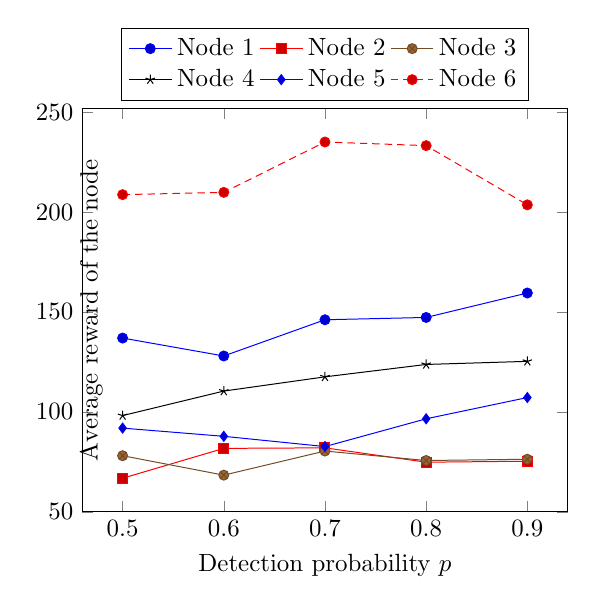
\begin{tikzpicture}[scale=0.9]
\begin{axis}[
  xlabel={Detection probability $p$},
  ylabel={Average reward of the node },
  y label style={at={(0.06,0.5)}},
  xtick={0.5,0.6,0.7,0.8,0.9,1.0},
  legend style={at={(0.5,1.2)},cells={align=right}, anchor=north,legend columns=3},
  grid style=dashed,
]

\addplot+[]
    coordinates {
(0.5,136.927310407)(0.6,127.960388869)(0.7,146.086472254)(0.8,147.235410707)(0.9,159.469537067)
};

\addplot+[]
    coordinates {
(0.5,66.7988560021)(0.6,81.7311837411)(0.7,82.0017291916)(0.8,74.8192160051)(0.9,75.3089759032)
};

\addplot+[]
    coordinates {
(0.5,78.0634438963)(0.6,68.3402801041)(0.7,80.4009699099)(0.8,75.6559526089)(0.9,76.2953944418)
};

\addplot+[]
    coordinates {
(0.5,98.1369317879)(0.6,110.402016785)(0.7,117.520015671)(0.8,123.721254753)(0.9,125.271778646)
};

\addplot+[]
    coordinates {
(0.5,91.8750388819)(0.6,87.764930694)(0.7,82.6400238592)(0.8,96.5305636149)(0.9,107.164379512)
};

\addplot+[]
    coordinates {
(0.5,208.678957661)(0.6,209.815036383)(0.7,235.024736742)(0.8,233.211114765)(0.9,203.573491786)
};

\legend{Node 1, Node 2, Node 3, Node 4, Node 5, Node 6}
\end{axis}
\end{tikzpicture}
% \label{fig:nodeimp_topo2_single}
\end{subfigure}
\begin{subfigure}{0.5\textwidth}
\caption{Scenario f)}
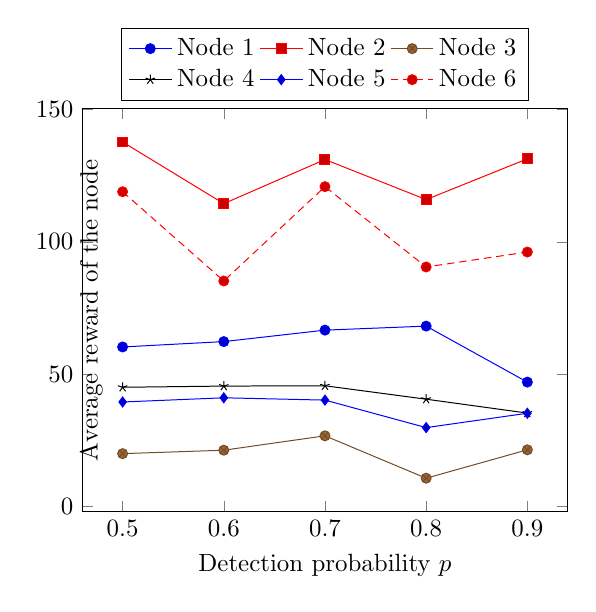
\begin{tikzpicture}[scale=0.9]
\begin{axis}[
  xlabel={Detection probability $p$},
  ylabel={Average reward of the node },
  y label style={at={(0.06,0.5)}},
  xtick={0.5,0.6,0.7,0.8,0.9,1.0},
  legend style={at={(0.5,1.2)},cells={align=right}, anchor=north,legend columns=3},
  grid style=dashed,
]

\addplot+[]
    coordinates {
(0.5,60.2573589594)(0.6,62.2897498389)(0.7,66.6189296773)(0.8,68.1381242941)(0.9,46.9747690794)
};

\addplot+[]
    coordinates {
(0.5,137.718591959)(0.6,114.415855021)(0.7,131.098099496)(0.8,115.956525872)(0.9,131.342366518)
};

\addplot+[]
    coordinates {
(0.5,19.9434781525)(0.6,21.2453007497)(0.7,26.6861654702)(0.8,10.6570889308)(0.9,21.3953375637)
};

\addplot+[]
    coordinates {
(0.5,45.028440798)(0.6,45.476076193)(0.7,45.5952834274)(0.8,40.5190352759)(0.9,35.2739320333)
};

\addplot+[]
    coordinates {
(0.5,39.4612966034)(0.6,41.0516205098)(0.7,40.1801733076)(0.8,29.7830035165)(0.9,35.211062317)
};

\addplot+[]
    coordinates {
(0.5,118.924992552)(0.6,85.1897448279)(0.7,120.841664824)(0.8,90.4846271321)(0.9,96.1337520102)
};

\legend{Node 1, Node 2, Node 3, Node 4, Node 5, Node 6}
\end{axis}
\end{tikzpicture}


% \label{fig:nodeimp_topo2_multiple}
\end{subfigure}
    \caption{Results for single and multiple attackers}
    \label{fig:mdp-results}
\end{figure}
% \clearpage

% }